\section*{Design Details}
\subsection*{First Approach}
\subsubsection*{Description}
The first filter approach utilized the block diagram shown in the project handout. This filter has three 8-bit multipliers, three 16-bit registers and two 16-bit adders. The design has a critical delay path of one multiplier and one adder. Truncation is performed at the end by simply discarding the 8 least-significant bits. A block diagram is shown in Figure \ref{fig:block1}. The full Verilog code can be found in the Verilog Code section.

\begin{figure}[h]
\begin{center}
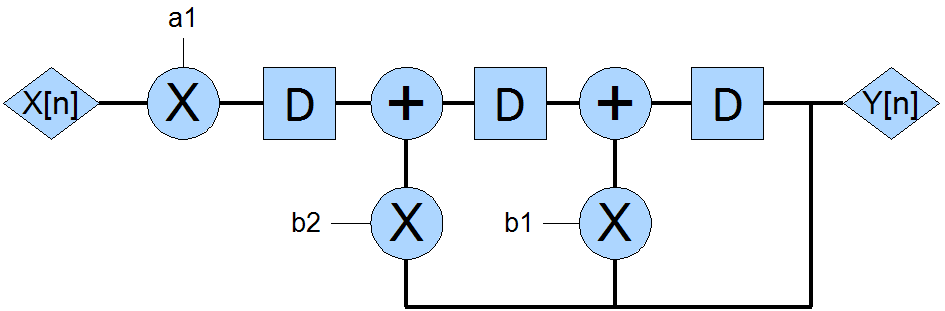
\includegraphics[scale=0.5]{block_one.png}
\end{center}
\caption{Block diagram of first filter design}
\label{fig:block1}
\end{figure}



This design does not utilize a reset signal. Instead, resetting is handled by modelling a weak pull-down in the registers. In the event that the input value is unknown or high impedence, the output value defaults to zero. This helps to reduce the port list and also internal routing required for this control signal. 

The overflow/underflow is handled by the logic found in the "always" block of add16.v. An if statement checks the XOR of the carry-in to the last bit with the carry-out of the last bit. If the result is 1, overflow or underflow has occurred. In order to determine which, the sign bits of the inputs must be checked. It is only necessary to check one of the inputs, since overflow or underflow can only occur when the inputs are either both positive or both negative. If the sign bit is found to be '0,' the output of the adder is +1. Otherwise the output is -1.

\lstset{language=verilog}
\lstinputlisting[caption=First approach overflow/underflow handling, label=lst:add16always]{plot1code/add16always.v}

\subsubsection*{Performance}
A Post-Place and Route Static Timing Analysis was performed on the design using Xilinx. The maximum delay path was found to be 17.408 ns, which correspondings to a maximum clock frequency of approximately 57.4 MHz. Details are shown in Table \ref{tab:timing1}. The filter performance was simulated with a provided Verilog testbench file. A Matlab plot of the filter input and output can be found on attached pages.

% Table generated by Excel2LaTeX from sheet 'Sheet1'
\begin{table}[h]
\caption{Xilinx Timing Report}
\begin{center}
\begin{tabular}{c|c}
           & Timing in (ns) \\
\hline
     Delay &   17.408  \\

Requrement &    100.000    \\

Data Path Delay &  17.408   \\
\end{tabular}  
\end{center}
\label{tab:timing1}
\end{table}


\subsubsection*{Discussion}
The Matlab plots of the filter input/output reveal that little-to-no attenuation of the high-frequency component of the signal takes place. It was not understood why this was occurring, even after discussion with one of the TA's. We decided to implement rounding truncation instead of discard truncation in the next design iteration in the hopes of improving the filter's attenuation performance.


\subsection*{Second Approach}
\subsubsection*{Description}
The approach of the second design was to measure the performance advantages/disadvantages of performing rounding truncation over a simple discarding of the eight least-significant bits. Because the method of rounding used involves an 8-bit adder, performing rounding will increase the critical path delay to a mulitplier and two adders. It was desired to measure exactly this performance hit, as well as any possible increase in the accuracy of the filter. A block diagram is shown in Figure \ref{fig:block2}.

\begin{figure}[h]
\begin{center}
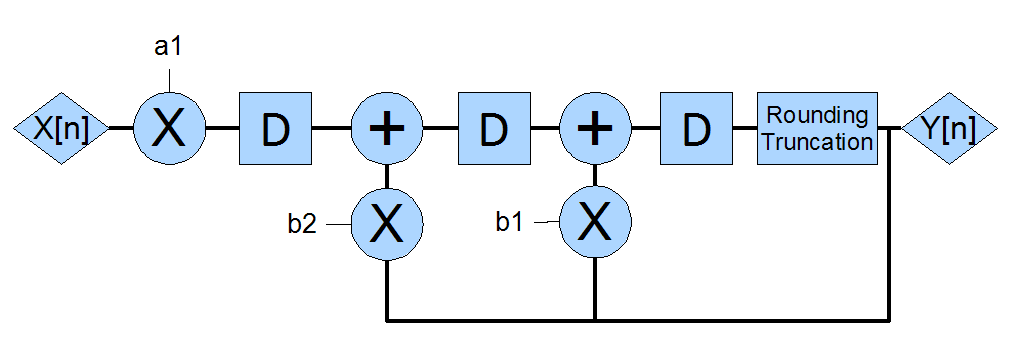
\includegraphics[scale=0.5]{block_two.png}
\end{center}
\caption{Block diagram of second filter design}
\label{fig:block2}
\end{figure}


The design is essentially the same, with the addition of add8.v, an 8-bit adder with exactly the same functionality as add16.v from the first design. This adder performs overflow/underflow handling in exactly the same way as previously described. In order to utilize this rounder, the following code was used to replace the "always" block of projfilt.v from the first design:


\lstinputlisting[caption=Round truncation code for second filter design, label=lst:add16always]{plot2code/projfiltalways.v}


\subsubsection*{Performance}
A Post-Place and Route Static Timing Analysis was performed on the design using Xilinx. The maximum delay path was found to be 18.684 ns, which correspondings to a maximum clock frequency of approximately 53.5 MHz. Details are shown in Table \ref{tab:timing2}. The filter performance was simulated with a provided Verilog testbench file. A Matlab plot of the filter input and output can be found on attached pages.

% Table generated by Excel2LaTeX from sheet 'Sheet1'
\begin{table}[h]
\caption{Xilinx Timing Report}
\begin{center}
\begin{tabular}{c|c}
           & Time (ns) \\
\hline
     Delay &     18.684 \\

Requrement &        100.000 \\

Data Path Delay &     18.538 \\
\end{tabular}  
\end{center}
\label{tab:timing2}
\end{table}


\subsubsection*{Discussion}
The Matlab plots revealed that the rounding truncation had no effect on the attenuation performance of the filter, but did however slightly reduce the noise from the first design approach. This design approach did reveal, however, that the rounding truncation incurred only a slight speed penalty from simple discarding, so it was decided to keep this feature in subsequent designs.



\subsection*{Third Approach}
The third design introduces an effort to decrease the critical path by placing registers after the multipliers. This so-called pipeline implementation utilizes three 16-bit registers, three 8-bit multipliers, two 16-bit adders, the same rounding truncation, but with an additional 8-bit register.  A block diagram is shown in Figure \ref{fig:block3}. The Verilog code for this design approach is same as the code for the fourth approach. The fourth approach merely replaces the adders.

\begin{figure}[h]
\begin{center}
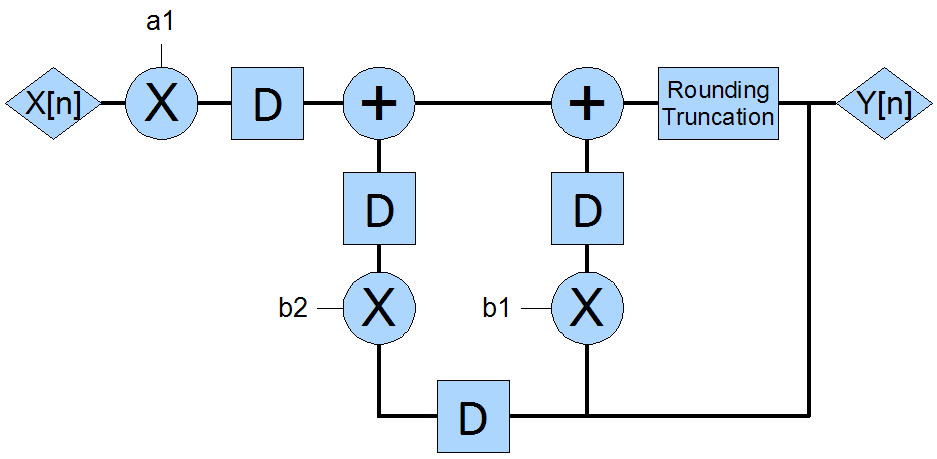
\includegraphics[scale=0.5]{block_three.png}
\end{center}
\caption{Block diagram of third/fourth filter design}
\label{fig:block3}
\end{figure}

For this approach, the truncation and overflow/underflow handling techniques utilized are the same as in design two. The key difference is in a re-design of the multiplier code and the main filter organization. The mult8.v code now includes a register to store the output of the multiplier, which enables the pipeline filter implementation.


\subsubsection*{Performance}
A Post-Place and Route Static Timing Analysis was performed on the design using Xilinx. The maximum delay path was found to be 17.962 ns, which correspondings to a maximum clock frequency of approximately 55.7 MHz. Details are shown in Table \ref{tab:timing1}. The filter performance was simulated with a provided Verilog testbench file. A Matlab plot of the filter input and output can be found on attached pages.

% Table generated by Excel2LaTeX from sheet 'Sheet1'
\begin{table}[h]
\caption{Xilinx Timing Report}
\begin{center}
\begin{tabular}{c|c}
           & Timing in (ns) \\
\hline
     Delay &  17.962   \\

Requrement &      100.000  \\

Data Path Delay &   17.951  \\
\end{tabular}  
\end{center}
\label{tab:timing3}
\end{table}

\subsubsection*{Discussion}
This result was peculiar because it demonstrated that our performance had actually \emph{decreased} with the pipeline implementation. This should not have happened. The critical path delay for this third approach is three adders, while the critical path delay for approach 2 is one multiplier and two adders. This means that our adder was actually slower than the multiplier.

After considering the design, we determined that this was because our adder implementation was a basic structural carry-ripple adder. This likely caused the adder to be much slower than it should have been. In order to achieve any performance gain, a re-write of the adders was necessary.


\subsection*{Fourth Approach}
\subsubsection*{Description}
The final design approach we attempted utilized the same pipeline principle as well as the same truncation and overflow/underflow handling as in the third approach. The only difference was the migration away from the carry-ripple adders from design approaches 1 and 2 to optimized Verilog adders. The complete code listing for the fourth approach can be found in the Verilog Code section.


\subsubsection*{Performance}
A Post-Place and Route Static Timing Analysis was performed on the design using Xilinx. The maximum delay path was found to be 11.445 ns, which correspondings to a maximum clock frequency of approximately 87.4 MHz. Details are shown in Table \ref{tab:timing4}. The filter performance was simulated with a provided Verilog testbench file. A Matlab plot of the filter input and output can be found on attached pages.

% Table generated by Excel2LaTeX from sheet 'Sheet1'
\begin{table}[h]
\caption{Xilinx Timing Report}
\begin{center}
\begin{tabular}{c|c}
           & Timing in (ns) \\
\hline
     Delay &   11.445  \\

Requrement &    100.000 \\

Data Path Delay & 11.369  \\
\end{tabular}  
\end{center}
\label{tab:timing4}
\end{table}

\subsubsection*{Discussion}
As expected, utilizing optimized adders greatly increased the performance of the circuit. The bottleneck was the adders. It should be noted here that the use of these library adders eliminated the overflow/underflow handling functionality. A look at the Matlab plots reveals, however, that this doesn't seem to have effected the attenuation performance of the filter at all. In fact, this design iteration has nearly exactly the same filter response as the last design iteration. The only change was a 57\% increase in the speed of the circuit.


